\documentclass[addpoints,11pt,a4paper]{exam}
\printanswers
\usepackage{amsmath, amssymb, amsthm}
\renewcommand{\rmdefault}{ppl} % rm
\linespread{1.05}        % Palatino needs more leading
\usepackage[scaled]{helvet} % ss
\usepackage{courier} % tt
\usepackage{eulervm} % a better implementation of the euler package (not in gwTeX)
\normalfont
\usepackage{caption}
\usepackage[T1]{fontenc}
\usepackage{mathrsfs}
\usepackage{comment}
\usepackage{graphicx}
\usepackage{ulem}
\usepackage{paralist}
\usepackage{psfrag}
\usepackage{fullpage}
\usepackage{fancybox}
\usepackage{ifthen}
\usepackage{hyperref}
\hypersetup{
    colorlinks=true,
    linkcolor=blue,
    filecolor=magenta,      
    urlcolor=blue,
}
\usepackage{marvosym}
\usepackage[export]{adjustbox}
\extrawidth{1in}
\usepackage{multicol}
\setlength{\columnsep}{.001cm}
\newcommand{\twopartdef}[4]
{
	\left\{
		\begin{array}{ll}
			#1 & \mbox{if } #2 \\
			#3 & \mbox{if } #4
		\end{array}
	\right.
}
\newcommand{\G}{\mathcal{G}}
\newcommand{\fH}{\mathcal{H}}
\newcommand{\M}{\mathcal{M}}
\title{CS6730 : Assignment 1}
\author{Instructor and TAs}
\date{Release: 26th Feb 2019; {\bf Due: Mar 7th, 11.59pm}}

\begin{document}
\maketitle
\noindent\rule{\textwidth}{1pt}
\begin{itemize}
    \item Submit to {\bf GradeScope a single LaTeX-generated pdf file} containing your solutions. Please type your answers in the solutions blocks in the source LaTeX file of this assignment. 
    \item The final question worth half overall points is a programming assignment that asks for (a) the formulas you used, (b) a well-documented code you wrote, and (c) submission of predictions from your code to a kaggle competition. 
    \item You are encouraged to collaborate/discuss with other students on this assignment, but write your solutions/code in your own words.
\end{itemize}
\noindent\rule{\textwidth}{1pt}

\begin{questions}
\question[6]{\sc [How tree-like are you?]} 
Let $H$ be an undirected graph with $n$ nodes. Let $T(H)$ be the set of all chordal graphs with $n$-nodes that contain all edges in $H$. The tree width of $H$ is defined as $\text{min} \{ \text{Max-Clique}(H')-1:H'\in T(H)\}$. 
\begin{parts}
\part[4] What is the tree-width of the $n\times n$ grid graph containing $n^2$ nodes?  Give proof.  (Hint: Answer scales linearly with $n$.)
%\begin{solution}
%\end{solution}
\part[2] What is the tree width of the cycle graph with $n$ nodes? Give proof. (Hint: Answer does not depend on $n$.)
%\begin{solution}
%\end{solution}
\end{parts}

\question[7]{\sc [Naive gets disoriented]}
\begin{parts}
\part[1] Give the MN structure and distribution for the Naive Bayes model, with the class label \textit{Y} taking values in the set $\{1,2, \ldots,n\}$ and feature values $X_1,\ldots,X_n$ taking values in $\{0,1\}$.
%\begin{solution}
%\end{solution}
\part[4] Give two distinct settings of the factors in the Markov network, so that $P(X_i=1|Y=j)$ = 0.9 if i = j and 0.1 otherwise.
%\begin{solution}
%\end{solution}
\part[2] One operation on MNs that arises in many settings (including variable elimination) is the marginalization of some node in the network. Give the minimal MN I-map for just the set of feature random variables $X_1,\ldots,X_n$ and also the form of any distribution $P$ that factorizes over such a network.
%\begin{solution}
%\end{solution}
\end{parts}

\question[7]{\sc [Moral sound of (d)sep]} 
Let $\G$ be a Bayesian Network DAG over $\mathcal{X}$, and let $\fH=\M[\G]$ be the moralized version of G. Let $X,Y,Z$ be {\bf any subsets} of $\mathcal{X}$. Then, state whether these statements are true or false, and briefly justify why. You can use the "Student" BN shown in figure below to obtain counter-examples or proof intuitions. 
\\(Note: This question provides tools for thinking about d-sep criteria in terms of the simpler sep criterion by moralization of the appropriate graph. This helps prove soundness of d-sep (which we only argued intuitively in class using all three-node DAGs) using soundness of sep (which is much easier to prove, as shown in class)]].
\begin{parts}
\part[1] Is ``X and Y are d-separated given Z in G if and only if X and Y are separated given Z in H''? 
%\begin{solution}
%\end{solution}
\part[2] Let $U = X \cup Y \cup Z$, and $\G'=\G[U \cup {\sc Ancs}_U]$ be the induced sub-graph over $U$ and its ancestors. Is ``$X$ and $Y$ are d-separated given $Z$ in $\G$ if and only if $X$ and $Y$ are d-separated given $Z$ in $\G'$''?
%\begin{solution}
%\end{solution}
\part[4] Consider same definitions as in (b) and let $\fH' = \M[\G']$. Is ``$X$ and $Y$ are d-separated given $Z$ in $\G'$ if and only if $X$ and $Y$ are separated given $Z$ in $\fH'$''?
%\begin{solution}
%\end{solution}
\end{parts}
\begin{center}
    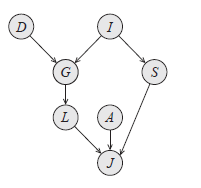
\includegraphics[width=0.3\textwidth]{assignment1-qn4.png}
\end{center}

\question[20]{\sc [Naive reorientation and upgrade]}
This programming assignment involves building Naive Bayes (NB) vs. Bayesian Network (BN) classifiers for detecting heart attack using cardiac images. Specifically, for the NB classifer and the BN classifier (whose structure is specified below), we ask for:
\begin{parts}
\part[5] formulas you used for (i) estimating conditional probability tables (CPTs' parameters) in the training step; and (ii) the log conditional probability of a class given all features in the testing step; and
%\begin{solution}
%\end{solution}
\part[15] (i) accuracy on the test set, obtained by submitting your code implementing each of the two classifiers to this \href{https://www.kaggle.com/t/f7ff0273602543fab4251ea052dc8e9b}{kaggle~competition~link}, and (ii) source-code listing of your well-documented code implementing the two classifiers in a language of your choice. The final submission to kaggle should be your best-performing classifier code. 
%\begin{solution}
  %Put accuracy of your two classifiers as reported by kaggle here.
  % 
  %\begin{lstlisting}
  %Put your code here.
  %\end{lstlisting}
%\end{solution}
\part[10] (Extra Credit worth 2.5\% of overall course marks) If you can modify the BN structure to get a better-performing classifier, please submit that BN classifier's predictions to kaggle, and mention here how you arrived at its structure to get extra credit.
%\begin{solution}
%\end{solution}
\end{parts}

\textbf{Detailed Instructions:}\\
A SPECT (Single Proton Emission Computed Tomography) scan of the heart is a noninvasive nuclear imaging test. Doctors use SPECT images to diagnose coronary artery disease and to detect if a heart attack occurred.
\begin{figure}[ht]
  \centering
  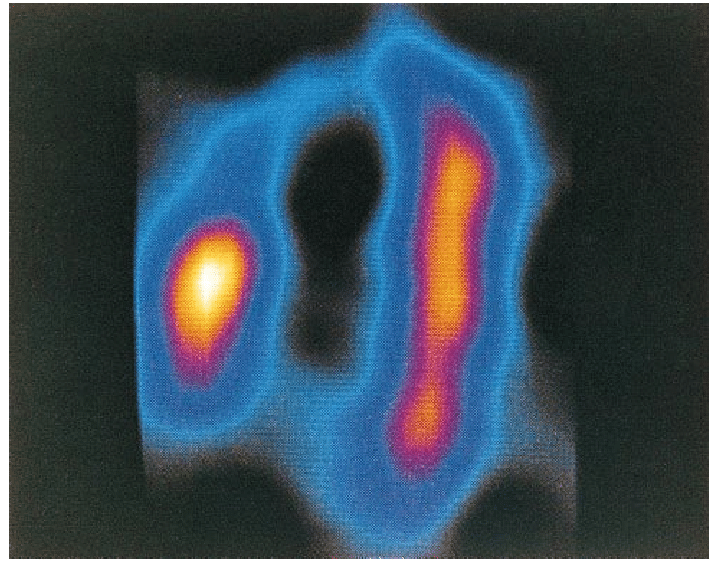
\includegraphics[width=3cm,height=3cm]{spect.png}
    \caption*{SPECT image of a normal heart.}
    \label{fig:spect}
\end{figure}

You will classify patients based on their cardiac SPECT images. Each patient will be classified into one of two categories: normal (zero) and abnormal (one). Each SPECT image was pre-processed to extract multiple features. As a result, 22 binary features were created for each patient from their SPECT image. Your task is to build classifiers based on this data, and then use it to predict if a patient is normal or not.

\textbf{Naive Bayes Classifier}
\begin{itemize}
    \item Binary Classification: Your program is intended for binary classification (i.e., classify patients as zero or one).
    \item Assume both the classes have same prior.
    \item Add-one Smoothing: To avoid any zero-count issues, use Laplace estimates (pseudocounts of 1) when estimating all probabilities. That is, 
    \begin{equation*}
        P(Y=y) = \frac{\#(y)+1}{\#(instances)+d}
    \end{equation*}
    where \#(y) denotes the number of instances having Y = y and d denotes the number of distinct values in Y  \href{https://en.wikipedia.org/wiki/Additive_smoothing}{[ref]}.
    \item Logs: Convert all probabilities to log probabilities to avoid underflow problems, using the natural logarithm.
    \item To break ties, classify as one (abnormal).
\end{itemize}

\textbf{Bayesian Network Classifier}
\begin{itemize}
    \item All the points same as the Naive Bayes Classifier.
    \item Structure: All features depend on class variable (same as naive bayes).  Along with that, both feature 8 (V8) and feature 9 (V9) are dependent on feature 16 (V16).
\end{itemize}

\textbf{Skeleton Code}\\
The code should have these functions:
\begin{itemize}
    \item NBfit
    \begin{itemize}
        \item Load the training data (train.csv). 
        \item Separate the classes and calculate the individual conditional probabilities for each feature given class.
    \end{itemize}
    \item NBeval
    \begin{itemize}
        \item Load the testing data (test.csv).
        \item Separate the actual class labels.
        \item For each sample point in test data, calculate the log conditional probability of class given the sample point.
        \item Assign each sample point to the class having high probability.
        \item Use the Accuracy function to evaluate the NB classifier.
    \end{itemize}
    \item BNfit
    \begin{itemize}
        \item Same as NBfit, but the individual conditional probabilities will change according to the BN.
    \end{itemize}
    \item BNeval
    \begin{itemize}
        \item Same as NBeval.
    \end{itemize}
\end{itemize}

\end{questions}
\end{document}